\subsection{Evaluation}
\label{sec:evaluation}

\todo{Short intro, one we have all the components of our evaluation}

\subsubsection{Response Time}
\label{sec:evaluation:response-time}

The protocol employed by the \textit{Treetalker} is a simple two-way exchange of data, where the treetalker will send measurements to the associated cloud and wait for new configuration parameters.
If it does not receive a response to its data packet after a certain time, it assumes that the cloud is offline and falls back to repeating the message ad-infinitum.
Thus,in order to be a viable alternative to the first-party \textit{TTCloud}, the \textit{\ttt} needs to be able to respond to each received data-packet within reasonable time.

In order to compare the response time of our system versus the TTCloud, we used a test-setup of a single Treetalker, in combination with a passive sniffing node, which recorded all LoRa-traffic.

\begin{figure}
    \centering
    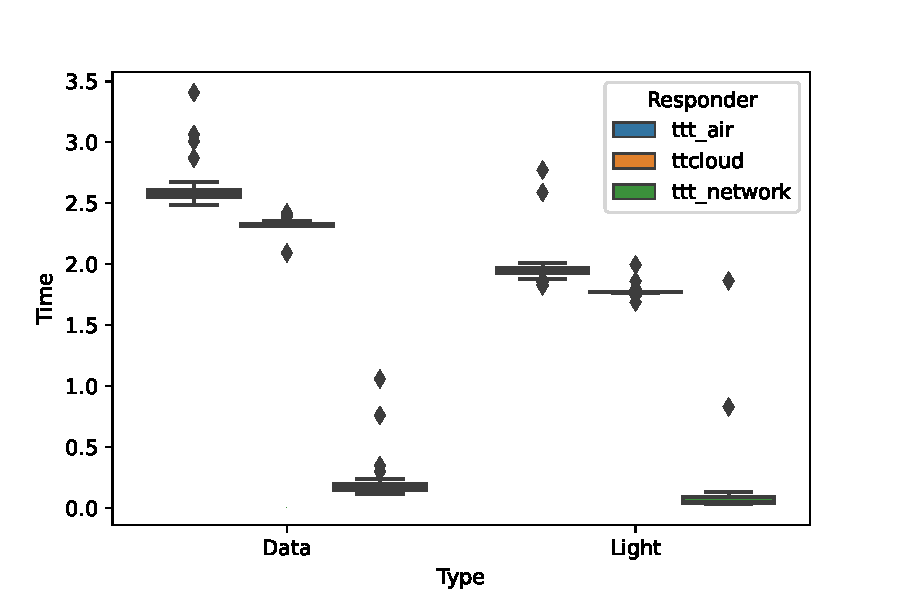
\includegraphics[width=.8\linewidth]{figures/response_times.pdf}
    \caption{Response time of both the first-party \textit{TTCLoud}, as well as the \textit{\ttt}.}
    \label{fig:evaluation:ttt_response}
\end{figure}

As can be seen in figure \ref{fig:evaluation:ttt_response}, the \ttt is capable delivering responses with a similar delay as the \textit{TTCloud}.
In fact, the actual time it takes to arrive at a decision and craft the reply-package is merely one-tenth of the total time, the other nine-tenths being the time neccessary to transmit the packet via LoRa.

It should be noted, that there are occasional outliers, wherein the {\ttt}'s will take a significantly longer time than average.
But even in these situations, the response-time is on-par with the TTCloud, rather than being higher.

\subsubsection{Protocol Overhead}
\label{sec:evaluation:overhead}

Another quality to consider is the overhead generated by our protocol.
Should our system generate a significant amount of additional overhead, it might prove unfeasible especially in bandwidth-constrained scenarios.

\paragraph{Treetalker-Gateway Communication}

Since the communication between the gateway and the Treetalker happens via LoRa, it is the most bandwidth-contrained.
Fortunately, since our gateway sends the exact same packets as a TTCloud would, there is no additional overhead generated on this communication interface.

\paragraph{Backend Communication}

The first-party TTCloud uses a proprietary communications protocol to send collected data to a centrlised server, there exists, to our knowledge, no publically accessible documentation as to the specific format of the protocol.
Furthermore, since the TTCloud sends data via GSM\footnote{The operator needs to qeuip each TTCloud with a SIM-Card, if they wish to benefit from automated data collection}, sniffing/reverse engineering of this protocol is unfeasible.

Our system uses the \textit{MQTT} message-broker protocol for all communication.
This protocol has been specifically designed for efficiency, that is low round-trip-times and little overhead.
To be precise, a MQTT \texttt{PUBLISH} generates a mere 15 bytes of overhead\cite{MQTT}, while a typical HTTP-request will have a header-size of 700-800 bytes\cite{SPDY}.

Packets are transmitted to the backend via MQTT, using the same compact binary serialsied format (encoded as \textit{base64}) as when transmitted via LoRa.

It is therefore highly unlikely that the data transmission from the TTCloud to the proprietary cloud service would have a significant lower overhead as our system.
Though for the aforementioned reason, we are unfortunately unable to give a precise, quantitative comparison.

\paragraph{Anomaly Detection}

To evaluate whether the anomaly-detection functions as intended, we drew upon real-world data gathered by a Treetalker-deployment, which was created as part of the \textit{Nature 4.0} project of the University of Marburg.
This deployment is comprised of 100 Treetalker which were set up in a university-owned parcel of forest and has been continually gathering sensor data for the past 2 years.

The evaluation was performed by injecting historical data into the policy-engine in chronological order, thus simulating a replay of the 2 year data-gathering-process.

\begin{table}
    \centering
    \begin{tabular}{l | c | c | c | c}
         Type & Position & Movement & Stem Temperature & Air Temperature  \\ \hline
         Anomalous & 2182 & 108 & 443 & 0 \\
         Critical & 6313 & 105 & 183 & 1
    \end{tabular}
    \caption{Anomalous and critical events found in historical data}
    \label{tab:evaluation:anomalies}
\end{table}

As becomes obvious from table \ref{tab:evaluation:anomalies}, the vast majority of events are produced by the accelerometer, and more specifically by the values denoting the sensor's position.

Further investigation of the data revealed that this seems to be due to a systematical fault in either the installed sensor itself, or the method in which this sensor is queried by the onboard electronics.

\begin{figure}
    \centering
    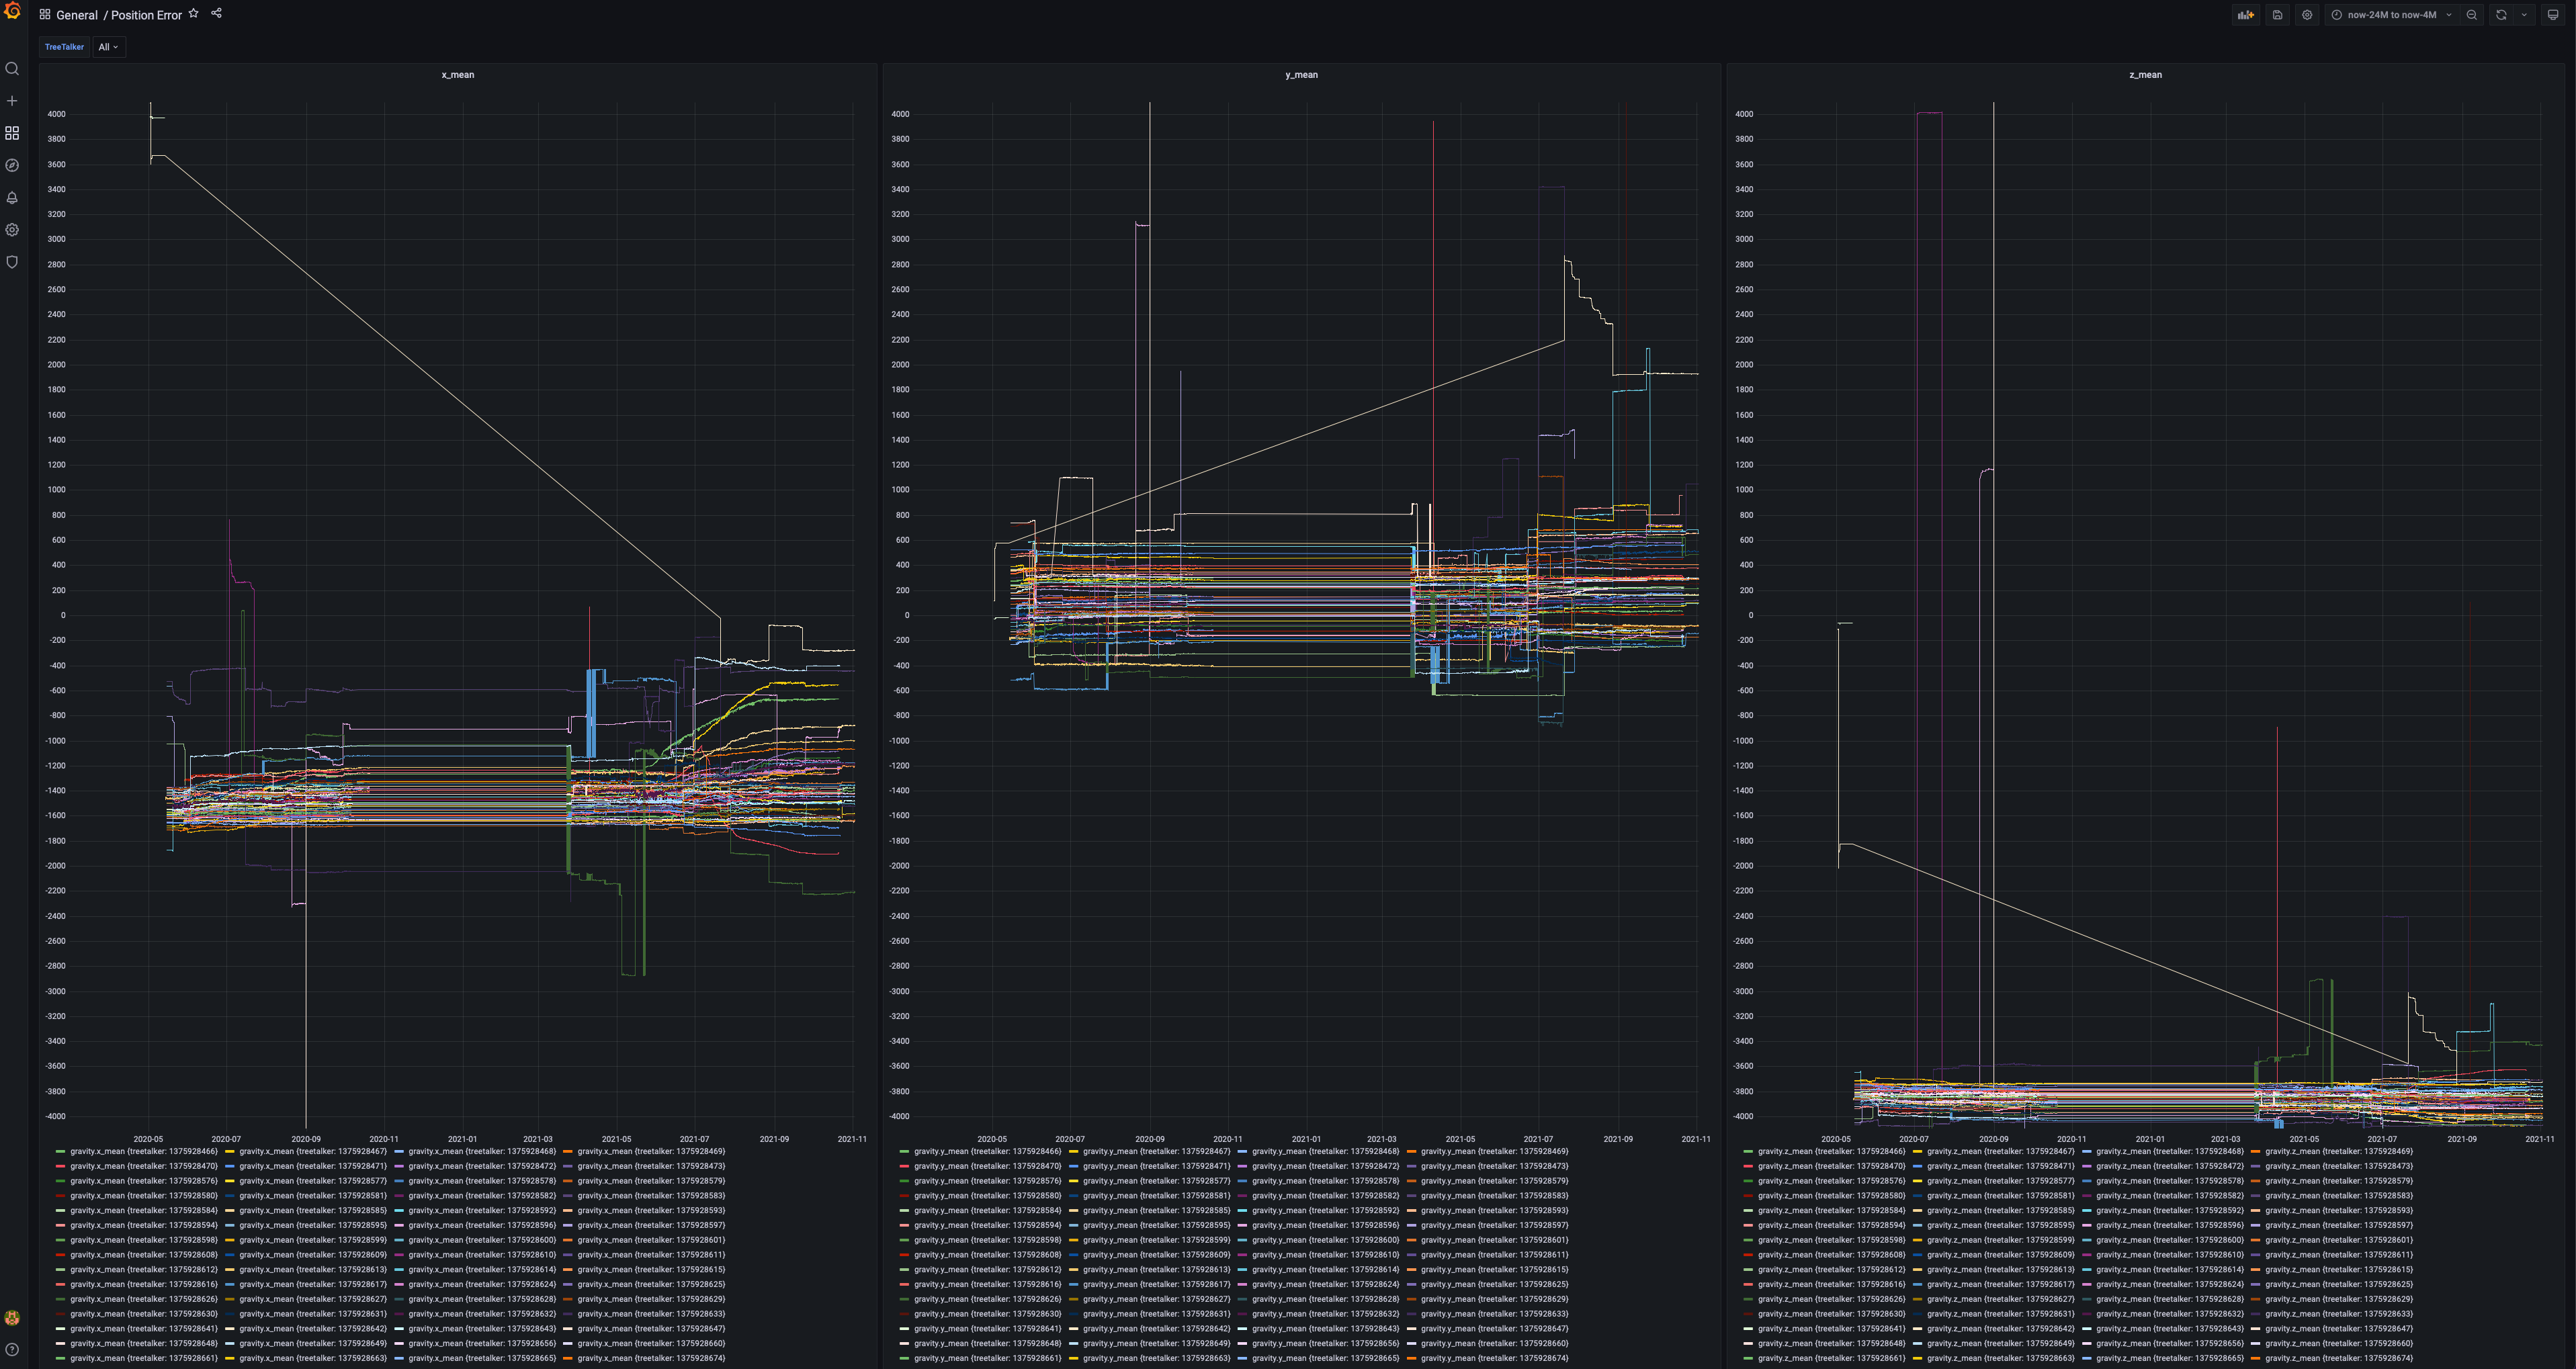
\includegraphics[width=.8\linewidth]{figures/TTT_position_data.png}
    \caption{Treetalker position data.}
    \label{fig:evaluation:position-data}
\end{figure}
